\lab{Optimization with Scipy}{scipy.optimize}
\label{lab:Optimization1}
\objective{Introduce some of the basic optimization functions available in \li{scipy.optimize}}

The Optimize package in Scipy has several functions for minimizing, root finding, and curve fitting. Here we will cover the usage of many of these functions.
You can learn about all of the functions at \url{http://docs.scipy.org/doc/scipy/reference/optimize.html}.

First we will test out a few of the minimization algorithms on the Rosenbrock Function, which is defined as
\[
f(x,y) = (1-x)^2 + 100(y-x^2)^2.
\]
The Rosenbrock function is commonly used when evaluating the performance of an optimization algorithm.
Reasons for this include the fact that its minimizer is found in a curved valley, and so minimizing the function is non-trivial.
See Figure \ref{opt:rosenbrock}.
The Rosenbrock function is included in the optimize package (as \li{rosen}), as well as its gradient (\li{rosen_der}) and its hessian (\li{rosen_hess}).

\begin{figure}
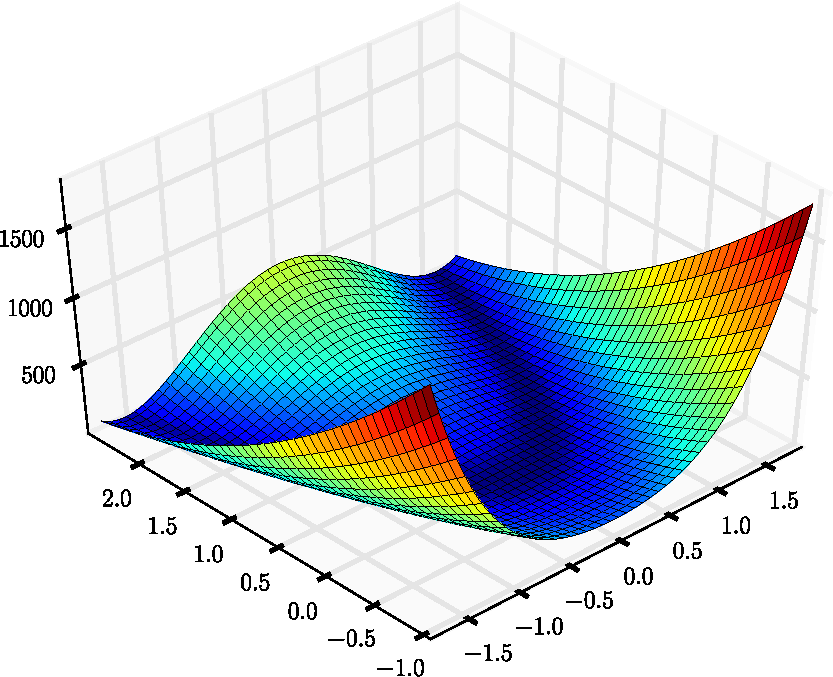
\includegraphics[width=\textwidth]{Rosenbrock.pdf}
\caption{$f(x,y) = (1-x)^2 + 100(y-x^2)^2$}
\label{opt:rosenbrock}
\end{figure}

We will use the \li{minimize} function and test each of its algorithms (specified by the keyword argument ``method" -- see the documentation page for \li{minimize}).
Note that there are also several functions such as \li{fmin} and \li{fmin_powell}. These are equivalent to using the \li{minimize} function with the specified method.

For each algorithm, you need to pass in a callable function object for the Rosenbrock function, as well as a NumPy array giving the initial guess.
For some algorithms, you will additionally need to pass in the jacobian or hessian.
You may recognize some of these algorithms, and several of them will be discussed in greater detail later. For this lab, you do not need to understand how they work, just
how to use them.

\begin{problem}
Import the \li{scipy.optimize} module as \li{opt}. Now use the \li{opt.minimize} function to find the minimum of the Rosenbrock function.
Test Nelder-Mead, Powell, CG, BFGS, Newton-CG, Anneal, L-BFGS-B, TNC, COBYLA, SLSQP.

The Newton-CG method takes in the jacobian and can take in the hessian. Test it with and without the hessian.
Part of the output of \li{opt.minimize} is the number of iterations each algorithm took (sometimes outputted as \li{nit}).
Start with the initial guess \li{x_0 = np.array([4., -2.5])}.
Which algorithm(s) take(s) the least number of iterations?
Which of the algorithms fail to find the (correct) minimum of the Rosenbrock?
For your solution, print the answers to these two questions.

As an example, we'll minimize the Rosenbrock with the Nelder-Mead method.
\begin{lstlisting}
>>> import numpy as np
>>> from scipy import optimize as opt
>>> x0 = np.array([4., -2.5])
>>> opt.minimize(opt.rosen, x0, method='nelder-mead', options={'xtol': 1e-8})
  status: 0
    nfev: 184
 success: True
     fun: 2.4359782685672914e-18
       x: array([ 1.,  1.])
 message: 'Optimization terminated successfully.'
     nit: 96
\end{lstlisting}
The printed output gives you information on the performance of the algorithm. In particular, the line \li{x: array([ 1.,  1.])} gives the obtained minimizer, and the final
line \li{nit: 96} gives the number of iterations.
\end{problem}

In the realm of optimization, convex functions are the most well-behaved, as any local minimum is a global minimum.
However, in practice one must frequently deal with non-convex functions, and sometimes we need pick the global minimum out of many local minima.

For example, consider the function
%This is the crazy function that I came up with to stump the algorithms
\[
z = r^2 (1+ \sin^2(4r)),
\]
where
\[
r = \sqrt{(x+1)^2 + y^2}.
\]
Essentially, this is a wavy crater offset from the origin by 1 along the $x$ axis (see Figure \ref{opt:multimin}).
\begin{figure}
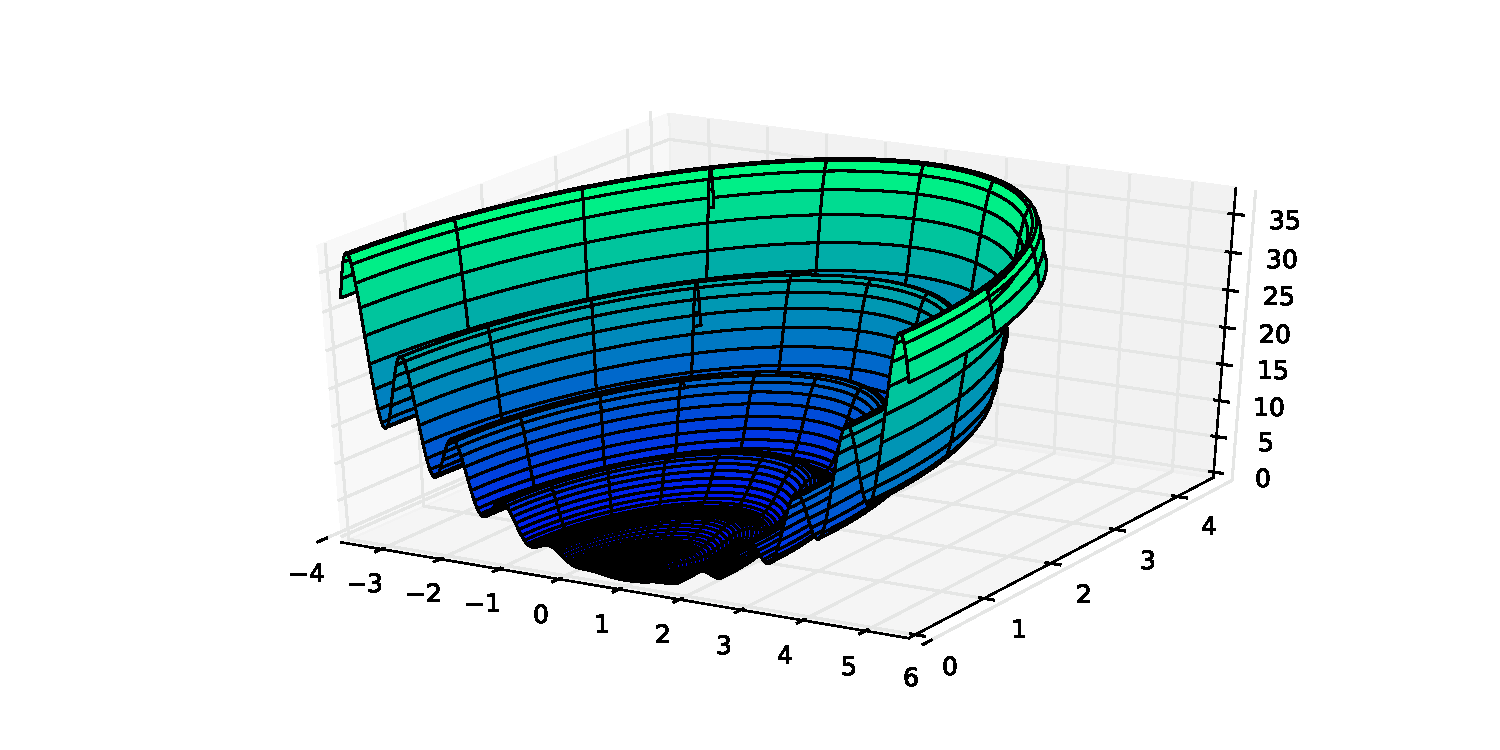
\includegraphics[width=\textwidth]{ManyMinima.pdf}
\caption{$z = r^2 (1+ 2\sin^2(4r))$}
\label{opt:multimin}
\end{figure}
The presence of many local minima proves to be a difficulty for the minimization algorithms.

For example, if we use the \li{opt.fmin} function (which employs the Nelder-Mead method), the algorithm fails to find the global minimum, and instead comes to rest on a local minimum.
\begin{lstlisting}
>>> def multimin(x):
>>>     r = np.sqrt((x[0]+1)**2 + x[1]**2)
>>>     return r**2 *(1+ np.sin(4*r)**2)
>>>
>>> x0 = np.array([-2, -2])
>>> res = opt.fmin(multimin, x0, xtol=1e-8, disp=True)
Optimization terminated successfully.
         Current function value: 5.488169
         Iterations: 56
         Function evaluations: 132
>>> print res
[-2.03513929 -2.08611595]
>>> print multimin(res)
5.48816865696
>>> print multimin([-1,0])
0.0
\end{lstlisting}

However, SciPy does have some tools to help us with these problems. Specifically, we can use the \li{opt.basinhopping} function.
Conceptually, most of the minimizing algorithms use the derivative of the function to search in a downhill direction for potential minimizers.
Often they overshoot the minimum and later backtrack. You can think of it as a ball rolling down a hill into a valley.
At first, the momentum of the ball carries it across the valley floor and partially up the other wall, only to roll back into the valley.
Slowly the ball loses momentum as it repeatedly overshoots and backtracks. Eventually the ball comes to rest at the bottom of a valley -- hopefully the lowest valley.
However, if there are many valleys (or local minima), the ball can get stuck in one that's not the lowest.
The \li{opt.basinhopping} function uses the same minimizing algorithms (in fact, you can tell it whatever minimizing algorithm you can pass to \li{opt.minimize}).
However, once it settles on a minimum, it hops to a new point in the domain (depending on how we set the ``hopping" distance) that hopefully lies outside of the valley
or basin belonging to the current local minimum.
It then searches for the minimum from this new starting point, and if it finds a better minimizer, it repeats the hopping process from this new minimizer.

\emph{Only Scipy Version 0.12+ has \li{opt.basinhopping}. In earlier versions, such as 0.11, you won't find it.}
%I've seen a real cool animation of this -feasible to do in python?
\begin{problem}

Look at the documentation for the \li{opt.basinhopping} function online and use it to find the global minimum of our \li{multimin} function with \li{x0 = np.array([-2, -2])}.
Use the same \li{Nelder-Mead} algorithm with the same \li{xtol}. Call it with \li{opt.basinhopping(multimin, x0, stepsize=0.5, minimizer_kwargs=\{'method':'nelder-mead'\})}.
Try it first with \li{stepsize=0.5} and then with \li{stepsize=0.2}. Why doesn't it find the minimum the second time? Print your answer to this question, and
return the minimum value the of the function with \li{stepsize=0.2}.

\end{problem}

The \li{optimize} package also has functions useful in root-finding.
The next example, taken from the online documentation, solves the following nonlinear system of equations using \li{opt.root}.

\[
\begin{bmatrix}
	x_{0} + 1/2 ( x_{0} - x_{1} )^{3} - 1 \\
	1/2(x_{1}-x_{0})^{3} + x_{1}
\end{bmatrix} =
\begin{bmatrix}
	0 \\
	0
\end{bmatrix}.
\]

\begin{lstlisting}
>>> def func(x):
>>>     return [x[0] + 0.5 * (x[0] - x[1])**3 -1.0,
>>>             0.5 * ( x[1] - x[0])**3 + x[1]]
>>> def jac(x):
>>>     return np.array([[1 + 1.5 * (x[0] - x[1])**2,
>>>                     -1.5 * (x[0] - x[1])**2],
>>>                     [-1.5 * (x[1] - x[0])**2,
>>>                     1 + 1.5 * (x[1] - x[0])**2]])
>>> sol = opt.root(func, [0, 0], jac=jac, method='hybr')
>>> print sol.x
[ 0.8411639  0.1588361]
>>> print func(sol.x)
[-1.1102230246251565e-16, 0.0]
\end{lstlisting}

\begin{problem}
Find the roots of the system
\[
\begin{bmatrix}
	-x+y+z \\
	1+x^3-y^2+z^3\\
	-2-x^2+y^2+z^2
\end{bmatrix} =
\begin{bmatrix}
	0 \\
	0 \\
	0
\end{bmatrix} .
\]
Return the values of $x,y,z$ as an array.
\end{problem}



As with \li{opt.minimize}, \li{opt.root} has more than one algorithm for root finding.
Here we have used the \li{hybr} method. There are also several algorithms for scalar root finding. See the online documentation for more.
%we still have curve fitting
%least squares programming -- but it seems that it's already been done in Volume One

SciPy also has methods for curve fitting wrapped by the \li{opt.curve_fit} function.
Just pass it data and a function to be fit. The function should take in the independent variable as its first argument and
values for the fitting parameters as subsequent arguments.
Examine the following example from the online documentation.
\begin{lstlisting}
>>> import numpy as np
>>> import scipy.optimize as opt

>>> #the function with which to create the data and later fit it
>>> def func(x,a,b,c):
>>>     return a*np.exp(-b*x) + c

>>> #create perturbed data
>>> x = np.linspace(0,4,50)
>>> y = func(x,2.5,1.3,0.5)
>>> yn = y + 0.2*np.random.normal(size=len(x));

>>> #perform the fit
>>> popt, pcov = opt.curve_fit(func,x,yn)
\end{lstlisting}
The variable \li{popt} now contains the fitted parameters and \li{pcov} gives the covariance of the fit.
See Figure \ref{opt:curve_fit} for a plot of the data and the fitted curve.

\begin{figure}
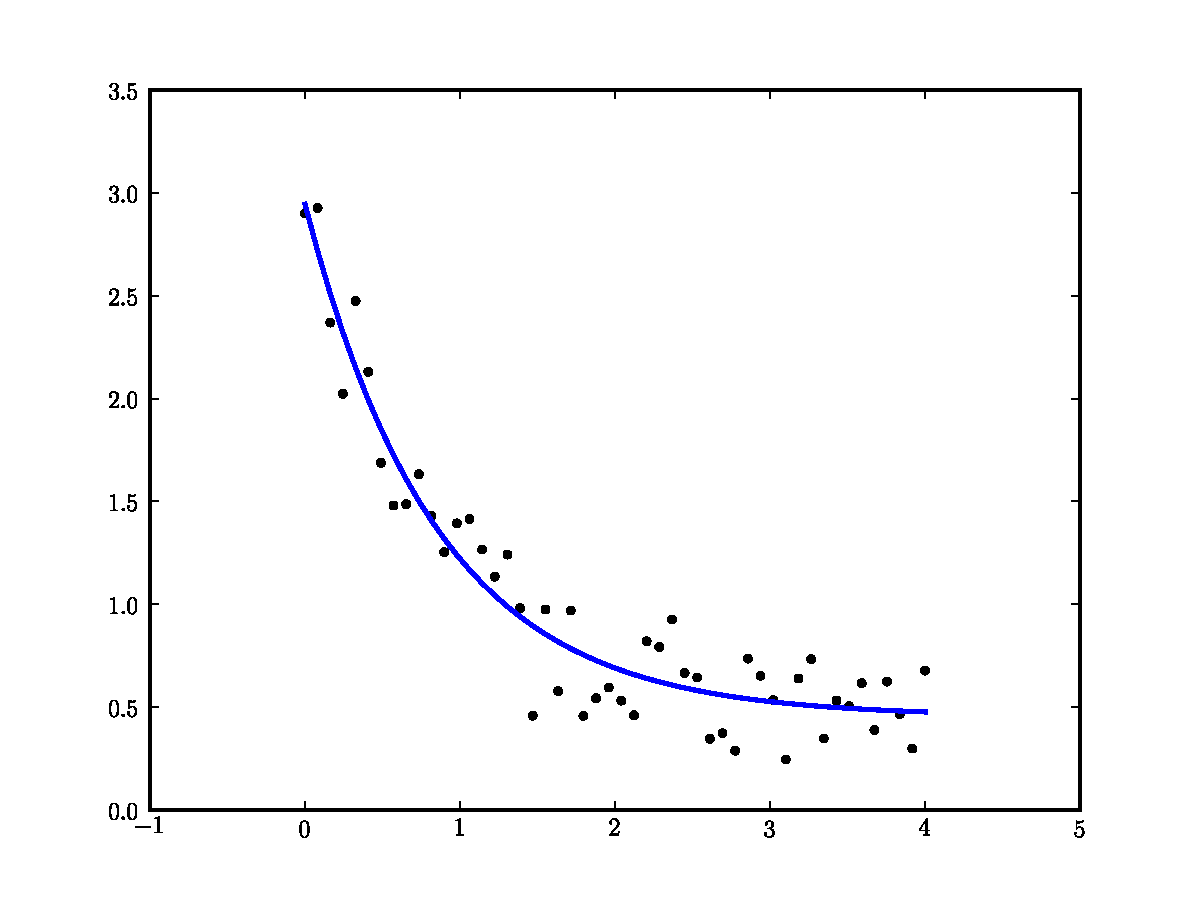
\includegraphics[width=\textwidth]{curve_fit.pdf}
\caption{Perturbed data graphed with the curve using the fitted parameters: $a=2.72$,  $b=1.31$, and $c=0.45$.}
\label{opt:curve_fit}
\end{figure}

\begin{problem}
Use the \li{opt.curve_fit} function to fit a heating curve to data obtained from a temperature sensitive diode embedded in a cylindrical aluminum block.
The data are in the file \li{heating.txt}. The first column is time and the second column is temperature in the Kelvin scale.
The temperature in the block was measured as it warmed from 290K up to 370K using a heating coil wound around the block attached to a
copper rod which sat in a cooling bath of liquid nitrogen.
Newton's law of cooling has the following form:
\[
T = T_{\infty} + \frac{P}{\gamma}+Ke^{-\frac{\gamma t}{C}},
\]\
where $T$ is the temperature (in Kelvin), $t$ is the time, $P$ is the power used to warm it (which here was 59.43 watts),
$T_{\infty}$ is the ambient temperature (290K), $\gamma$ is a coefficient of heat transfer through the copper rod,
$C$ is the total heat capacity of the block, and $K$ is a constant coefficient that depends on the initial conditions.
Use \li{opt.curve_fit} to find a fit to the data using $\gamma$, $C$, and $K$ as the fitting parameters.
Just so that you know that you are getting realistic values, $\gamma$ should be on the order of $10^{-1}$, $C$ on the order of $10^{2}$, and $K$ should be negative on the order of $10^{2}$.
Return your values for $\gamma$, $C$, and $K$ in a NumPy array of length 3.

See Figure \ref{opt:HeatingFit} for a plot of the data along with a fitted curve.

\begin{comment}
From the heat capacity you obtained in the fit you can calculate the specific heat capacity of the aluminum block by dividing the heat capacity by the mass of the block (about 300g). Is it close to the experimentally measured specific heat capacity of aluminum of 0.900 J/g K? From $\gamma$ you can also calculate the thermal conductivity of the copper rod using the formula $k=\gamma L/A$ where $L$ and $A$ are the length ($25.6mm$) and the cross-sectional area ($71.24mm^{3}$) of the rod. How does it compare to the experimentally measured thermal conductivity of $401 W/(m \dot K)$? Look at the covariance you got from the fit. Is the error due to the fit, noise in the data, or an error in the excremental setup?
\end{comment}
\end{problem}

\begin{figure}
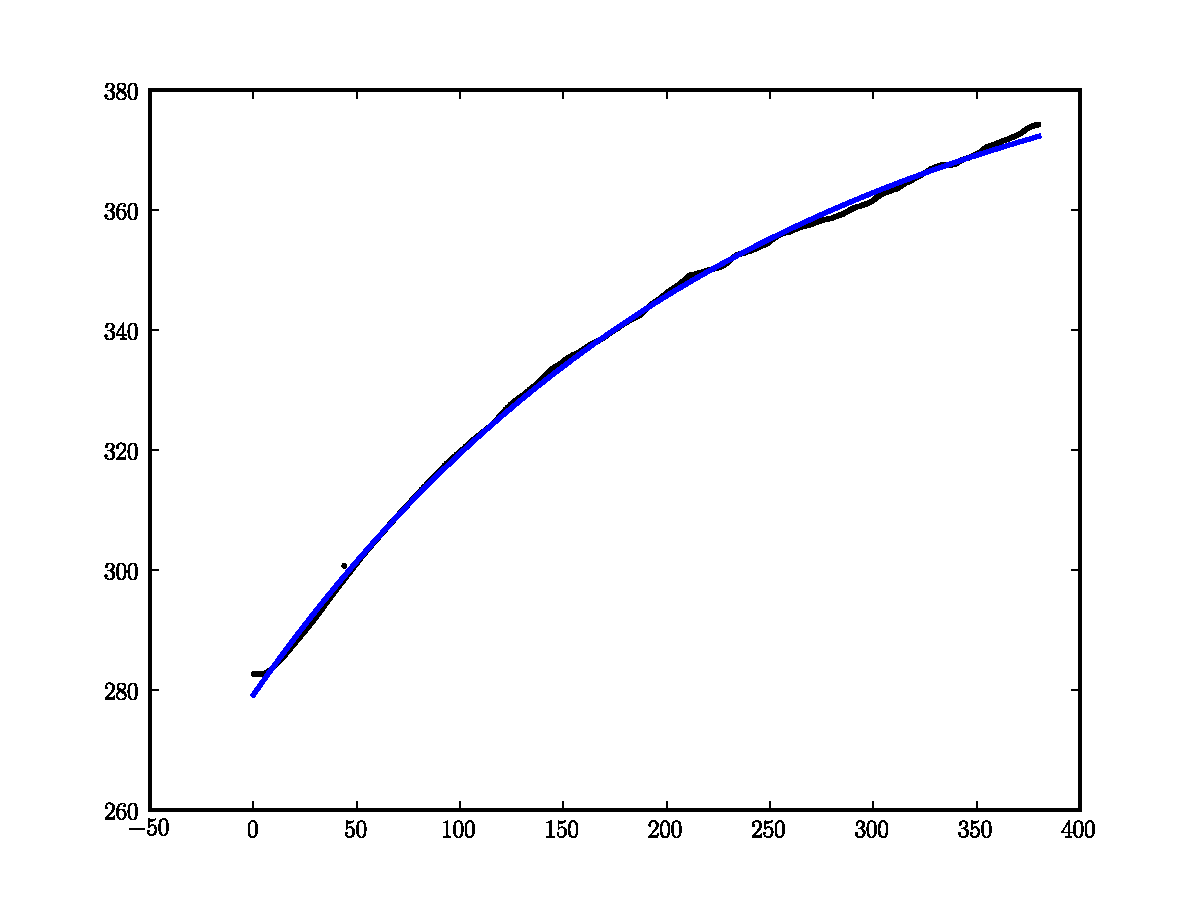
\includegraphics[width=\textwidth]{HeatingFit.pdf}
\caption{The black line is actually the data from \li{heating.txt} plotted as a scatter plot. It appears as a line because the data is very dense. The blue line is a fitted curve.}
\label{opt:HeatingFit}
\end{figure}

The \li{scipy.optimize} package has many other useful functions, and is a good first resource when confronting a numerical optimization problem. See the online documentation for further details.


